\documentclass[aps,prc,reprint]{revtex4-1}

\usepackage{siunitx}
\usepackage{amsmath}
\usepackage{mathtools}
% \usepackage{algorithm}
% \usepackage{algpseudocode}
% \usepackage{minted}
\usepackage{url}
\frenchspacing

\newcommand{\sddots}[0]{\ensuremath{\smash{\ddots}}}

% \usemintedstyle{xcode}


\begin{document}

\title{Project 2: Solving Schr\"odinger's equation for two electrons in a 3D harmonic oscillator well using Jacobi's rotation algorithm}
\author{Joshua Bradt}
\noaffiliation
\date{March 4, 2016}

\begin{abstract}
    Expressions for the Hamiltonian of one and two electrons trapped in a harmonic oscillator potential are derived. Jacobi's rotation algorithm for diagonalizing a system of equations is presented, and an implementation of this algorithm in C is used to find the first few eigenvalues and eigenfunctions of the system. The results are compared to results calculated by a function from the Armadillo linear algebra library \cite{Sanderson2010} and to an analytic solution \cite{Taut1993}. In both cases, the results calculated here and the results from other sources are in agreement. Finally, the performance of Jacobi's algorithm is measured and found to be much slower than the algorithm used by Armadillo.
\end{abstract}

\maketitle

\section{Introduction}
\label{sec:introduction}
    A commonly studied system in physics is that of the electron confined in a potential well of some sort. This arises in, for example, the study of quantum dots, quantum computing, and other areas of solid-state physics. \cite{courserepo} For the purposes of this work, we will consider the cases of one or two electrons confined by a harmonic oscillator potential, the theory of which is described in Section~\ref{sec:theory}. The one-electron case is a simple example of a particle interacting with an external potential, but the two-electron case is more complex due to the Coulomb repulsion between the two negatively charged particles. That being said, both of these cases admit analytic solutions. The solution to the one-electron problem is derived in most introductory quantum mechanics texts (e.g. \textcite[p. 351]{Shankar1994}), but an exact solution for the two-electron problem was only more recently found by \textcite{Taut1993}.

    Instead of analytic solutions, it is often easier to seek a numerical solution. One simple way to do this is Jacobi's rotation algorithm, which is derived in Section~\ref{sec:numsoln}. This method produces correct results, and is relatively easy to implement, but it is also quite inefficient, as shown in Section~\ref{sec:results}.

\section{Theory}
\label{sec:theory}

    \subsection{One electron case}
    \label{sub:oneelec}
        Assuming spherical symmetry, we can write the radial part of Schr\"odinger's equation for the confined electron in three dimensions as
        \begin{multline}
            -\frac{\hbar^2}{2m} \left( \frac{1}{r^2} \frac{d}{dr} r^2 \frac{d}{dr} - \frac{l(l+1)}{r^2} \right) R(r) +{} \\ V(r)R(r) = ER(r).  \label{eq:genschro}
        \end{multline}
        Here, $R(r)$ is the radial wave function of the electron, $l$ is the angular momentum, $V(r)$ is the confining potential, and $E$ is the energy. If we take the potential to be the three-dimensional harmonic oscillator potential,
        \begin{equation}
            V(r) = \frac{1}{2} m \omega^2 r^2,
        \end{equation}
        then the energies are known to be
        \begin{equation}
            E_{nl} = \hbar\omega \left( 2n + l + \frac{3}{2} \right)
        \end{equation}
        with principal quantum number $n=0,1,2,\dots$ and angular momentum quantum number $l=0,1,2,\dots$. \cite{Shankar1994}

        Next, make the substitution $R(r) = (1/r) u(r)$ in (\ref{eq:genschro}) to find
        \begin{equation*}
            -\frac{\hbar^2}{2m} \left( \frac{d^2}{dr^2} - \frac{l(l+1)}{r^2} \right) u(r) + V(r)u(r) = Eu(r).
        \end{equation*}
        If we set $l = 0$ and thereby neglect the centrifugal barrier term---which is effectively just an extra term in the potential---we can write this as
        \begin{equation*}
            -\frac{\hbar^2}{2m} \frac{d^2}{dr^2} u(r) + \frac{1}{2} m \omega^2 r^2 u(r) = Eu(r)
        \end{equation*}
        where $V(r)$ has been replaced with the expression for the harmonic oscillator potential introduced above. This can then be simplified by introducing the dimensionless variable $\rho = r / \alpha$ where $\alpha$ is an arbitrary constant with the dimensions of length:
        \begin{equation*}
            -\frac{\hbar^2}{2m\alpha^2} \frac{d^2}{d\rho^2} u(\rho) + \frac{1}{2} m \omega^2 \alpha^2 \rho^2 u(\rho) = Eu(\rho).
        \end{equation*}
        This can be rearranged to find
        \begin{equation*}
            -\frac{d^2 u}{d\rho^2} + \frac{m^2\omega^2\alpha^4}{\hbar^2} \rho^2 u(\rho) = \frac{2m\alpha^2}{\hbar^2} E u(\rho)
        \end{equation*}
        which suggests that we define $\alpha = \sqrt{\hbar / m\omega}$ and $\lambda = 2E / \hbar\omega$ to get
        \begin{equation}
            -\frac{d^2 u}{d\rho^2} + \rho^2 u(\rho) = \lambda u(\rho).  \label{eq:oneelecfinal}
        \end{equation}

    \subsection{Two-electron case}
    \label{sub:twoelec}
        The theory of the two-electron case is very similar to that laid out above in Section~\ref{sub:oneelec}. Begin with the radial part of Schr\"odinger's equation for the two electrons in a potential $V$:
        \begin{multline}
            \left( -\frac{\hbar^2}{2m} \frac{\partial^2}{\partial r_1^2} - \frac{\hbar^2}{2m} \frac{\partial^2}{\partial r_2^2} + V(r_1, r_2) \right) u(r_1, r_2) ={} \\ Eu(r_1, r_2).  \label{eq:twoelecbase}
        \end{multline}
        The potential $V$ must include the interaction of each electron with the well and the Coulomb repulsion between the two electrons. This can be written as
        \begin{equation*}
            V(r_1, r_2) = \frac{1}{2}m\omega^2 r_1^2 + \frac{1}{2}m\omega^2 r_2^2 + \frac{ke^2}{|\mathbf{r}_1 - \mathbf{r}_2|},
        \end{equation*}
        where $k = 1 / 4\pi\epsilon_0$.

        Equation \ref{eq:twoelecbase} can be simplified by introducing the electron separation distance $r = |\mathbf{r}_1 - \mathbf{r}_2|$ and the center-of-mass coordinate $R = (1/2)(\mathbf{r}_1 + \mathbf{r}_2)$. This substitution gives
        \begin{multline*}
            \left( -\frac{\hbar^2}{m}\frac{\partial^2}{\partial r^2} - \frac{\hbar^2}{4m}\frac{\partial^2}{\partial R^2} + \frac{1}{4}m\omega^2 r^2 +{} \right.\\\left. m\omega^2 R^2  + \frac{ke^2}{r} \right) u(r,R) = (E_r + E_R) u(r,R).
        \end{multline*}
        For simplicity, we'll neglect the center-of-mass motion. This leaves
        \begin{equation*}
            \left( -\frac{\hbar^2}{m}\frac{d^2}{dr^2} + \frac{1}{4}m\omega^2 r^2 + \frac{ke^2}{r} \right) u(r) = E_r u(r).
        \end{equation*}
        Like in the one-electron case, we can define a unitless variable $\rho = r / \alpha$ and write
        \begin{equation*}
            \left( -\frac{\hbar^2}{m\alpha^2}\frac{d^2}{d\rho^2} + \frac{1}{4}m\omega^2\alpha^2 \rho^2 + \frac{ke^2}{\alpha\rho} \right) u(\rho) = E_r u(\rho),
        \end{equation*}
        which can be rearranged to get the equation
        \begin{equation*}
            \left( -\frac{d^2}{d\rho^2} + \frac{m^2\omega^4\alpha^4}{4\hbar^2} \rho^2 + \frac{ke^2m\alpha}{\hbar^2\rho} \right) u(\rho) = \frac{m\alpha^2E_r}{\hbar^2} u(\rho).
        \end{equation*}
        Define $\alpha = \hbar^2 / mke^2$, $\omega_r^2 = m^2\omega^4\alpha^4 / 4\hbar^2$, and $\lambda = m\alpha^2E_r / \hbar^2$ to find
        \begin{equation}
            -\frac{d^2 u}{d\rho^2} + \omega_r^2 \rho^2 u(\rho) + \frac{1}{\rho} u(\rho) = \lambda u(\rho). \label{eq:twoelecfinal}
        \end{equation}

        Equation (\ref{eq:twoelecfinal}) is nearly identical to (\ref{eq:oneelecfinal}); the only difference is the replacement of the potential $V(\rho) = \rho^2$ from the one-electron case with the new two-electron potential $V(\rho) = \omega_r^2 \rho^2 + 1/\rho$. This implies that we can develop a numerical solution to the general equation
        \begin{equation}
            -\frac{d^2 u}{d\rho^2} + V(\rho) u(\rho) = \lambda u(\rho)  \label{eq:generaldiffeq}
        \end{equation}
        and then plug in the two different potentials to solve the one- and two-electron cases.


\section{Numerical solution}
\label{sec:numsoln}
    To solve (\ref{eq:generaldiffeq}) numerically, begin by expressing the second derivative using the finite difference equation
    \begin{equation}
        u''(\rho) = \frac{u(\rho + h) + u(\rho - h) - 2u(\rho)}{h^2} + O(h^2)  \label{eq:findiff}
    \end{equation}
    with step size $h$. For simplicity, define
    \begin{align*}
        u_i         &= u(\rho)       \\
        u_{i \pm 1} &= u(\rho \pm h) \\
        \rho_i      &= ih            \\
        V_i         &= V(\rho_i).
    \end{align*}
    Using these expressions and discretizing (\ref{eq:generaldiffeq}) between $\rho = 0$ and some arbitrary $\rho_\text{max}$ then yields
    \begin{equation*}
        -\frac{u_{i+1} + u_{i-1} - 2u_i}{h^2} + V_i u_i = \lambda u_i
    \end{equation*}
    for $i=0,1,\dots,N$ and $h = \rho_\text{max} / N$. Rearranging this equation gives
    \begin{equation*}
        - \frac{1}{h^2} u_{i+1} - \frac{1}{h^2} u_{i-1} + \left(\frac{2}{h^2} + V_i\right)u_i = \lambda u_i,
    \end{equation*}
    which suggests treating the problem as a system of linear equations
    \begin{equation}
        \mathbf{A}\mathbf{u} = \lambda \mathbf{u},
    \end{equation}
    where the tridiagonal matrix $\mathbf{A}$ is defined as
    \begin{equation}
        \begin{pmatrix}
            \frac{2}{h^2}+V_1 & -\frac{1}{h^2}    &                &        & \vphantom{\ddots} \\
            -\frac{1}{h^2}    & \frac{2}{h^2}+V_2 & -\frac{1}{h^2} &        & \vphantom{\ddots} \\
                              & -\frac{1}{h^2}    & \ddots         & \ddots &                   \\
                              &                   & \ddots         & \ddots & -\frac{1}{h^2}    \\
            \vphantom{\ddots} &                   &             & -\frac{1}{h^2} & \frac{2}{h^2}+V_{N-1} \\
        \end{pmatrix}
    \end{equation}
    and the vector $\mathbf{u} = \begin{pmatrix}u_1 & u_2 & \dots & u_{N-1}\end{pmatrix}^T$.

    \subsection{Jacobi's rotation algorithm}
    \label{sub:jacobi}
        One way to solve the system of linear equations we've found is by using Jacobi's rotation algorithm. This method iteratively applies similarity transformations to the matrix $\mathbf{A}$ until it becomes diagonal \cite{courserepo}. That is, for orthogonal matrices $\mathbf{S}_i$, the matrix is transformed as
        \begin{equation*}
            \mathbf{S}_m^T \mathbf{S}_{m-1}^T \dots \mathbf{S}_{1}^T \mathbf{A} \mathbf{S}_{1} \mathbf{S}_{2} \dots \mathbf{S}_{m} = \mathbf{D}
        \end{equation*}
        where the final matrix $\mathbf{D}$ is diagonal. Naturally, identical transformations must be applied to the eigenvector to maintain equality, but since the constant eigenvalue can be factored out of all of the matrix multiplications, these similarity transformations do not change the eigenvalues of the matrix. \cite{courserepo}

        Jacobi's rotation algorithm, in particular, chooses these orthogonal matrices to be
        \begin{equation}
            \mathbf{S} = \begin{pmatrix}
                1      & 0      & \dots  & 0           & \dots &  0         & \dots & 0\\
                0      & 1      & \dots  & 0           & \dots &  0         & \dots & 0\\
                \vdots & \vdots &        & \vdots      &       & \vdots     &       & \vdots \\
                0      & 0      & \dots  & \cos\theta  & \dots & \sin\theta & \dots & 0\\
                \vdots & \vdots &        & \vdots      &       & \vdots     &       & \vdots \\
                0      & 0      & \dots  & -\sin\theta & \dots & \cos\theta & \dots & 0 \\
                \vdots & \vdots &        & \vdots      &       & \vdots     &       & \vdots \\
                0      & 0      & \dots  & 0           & \dots & 0          & \dots & 1 \\

            \end{pmatrix},
        \end{equation}
        a generalized rotation matrix with elements
        \begin{equation*}
            S_{ij} = \begin{dcases}
                1           & i=j,\quad i,j \notin \{p,q\}  \\
                \cos\theta  & (ij=pp) \cup (ij=qq) \\
                \sin\theta  & ij=pq \\
                -\sin\theta & ij=qp \\
                0           & \text{elsewhere}.
            \end{dcases}
        \end{equation*}
        Note that the $\cos\theta$ elements are not necessarily along the diagonal of the matrix.

        The values of $\cos\theta$ and $\sin\theta$ can be found by looking at the elements affected by the transformation:
        \begin{equation*}
            \begin{pmatrix}
                b_{pp} & b_{pq} \\
                b_{qp} & b_{qq} \\
            \end{pmatrix}
            =
            \begin{pmatrix}
                c & -s \\
                s & c \\
            \end{pmatrix}
            \begin{pmatrix}
                a_{pp} & a_{pq} \\
                a_{qp} & a_{qq} \\
            \end{pmatrix}
            \begin{pmatrix}
                c & s \\
                -s & c \\
            \end{pmatrix}.
        \end{equation*}
        Here, we've defined $c\equiv\cos\theta$ and $s\equiv\sin\theta$. To make the matrix $\mathbf{A}$ diagonal, we want to make $b_{pq} = b_{qp} = 0$. Therefore, we carry out the matrix multiplication and find
        \begin{equation}
            b_{qp} = a_{pq}(c^2-s^2) + (a_{pp} - a_{qq}) cs = 0.  \label{eq:bqp}
        \end{equation}
        If we define
        \begin{gather}
            \tau = \frac{a_{qq} - a_{pp}}{2a_{pq}}  \label{eq:tau} \\
            t = \tan\theta = \frac{s}{c}
        \end{gather}
        then (\ref{eq:bqp}) can be rearranged and written as
        \begin{equation*}
            t^2 + 2\tau t - 1 = 0
        \end{equation*}
        which has roots
        \begin{equation*}
            t = -\tau \pm \sqrt{\tau^2 + 1} = \frac{1}{\tau \pm \sqrt{\tau^2 + 1}}.
        \end{equation*}
        To help prevent $t$ from diverging due to loss of numerical precision when $|\tau| \ll 1$, we choose the smaller of the two roots. Thus,
        \begin{equation}
            t = \begin{dcases}
                \frac{1}{\tau + \sqrt{\tau^2 + 1}} & \tau \geq 0 \\
                \frac{1}{\tau - \sqrt{\tau^2 + 1}} = \frac{-1}{-\tau + \sqrt{\tau^2 + 1}} & \tau < 0. \\
            \end{dcases}
            \label{eq:t}
        \end{equation}
        Knowing $t$ then gives values for $s$ and $c$ via trigonometric identities
        \begin{equation}
            c = \frac{1}{\sqrt{1 + t^2}} \quad \text{and}\quad s = tc, \label{eq:cs}
        \end{equation}
        and thereby defines the elements of the rotation matrix $\mathbf{S}$. Thus, the elements of the transformed matrix $\mathbf{B} = \mathbf{S}^T \mathbf{A} \mathbf{S}$ are
        \begin{align}
            b_{ip} &= ca_{ip} - sa_{iq}, \quad i \notin \{p, q\} \label{eq:bFirst}\\
            b_{iq} &= ca_{iq} + sa_{ip}, \quad i \notin \{p, q\} \\
            b_{pp} &= c^2 a_{pp} - 2csa_{pq} + s^2 a_{qq} \\
            b_{qq} &= c^2 a_{qq} + 2csa_{pq} + s^2 a_{pp} \\
            b_{pq} &= a_{pq}(c^2-s^2) + (a_{pp} - a_{qq}) cs = 0 \label{eq:bLast}
        \end{align}
        with equivalent transformations for the elements opposite the diagonal to maintain orthogonality. These equations are the basis of the Jacobi rotation algorithm.

        The algorithm itself consists of a few basic steps:
        \begin{enumerate}
            \item Find the largest off-diagonal element in $\mathbf{A}$. The indices of this element are $p$ and $q$.
            \item Calculate $\tau$ using (\ref{eq:tau}), $\tan\theta$ using (\ref{eq:t}), and $\cos\theta$ and $\sin\theta$ using (\ref{eq:cs}).
            \item Calculate the new matrix elements $b_{ij}$ using (\ref{eq:bFirst}--\ref{eq:bLast}).
            \item Check to see if the norm of the off-diagonal elements is less than some tolerance $\epsilon$. If not, repeat the process until it is.
        \end{enumerate}

\section{Results}
\label{sec:results}
    The algorithm described in Section~\ref{sec:numsoln} was implemented in C and run for both the one- and two-electron cases. This implementation can be found online in the repository at \cite{github} in the file \texttt{project2/src/jacobi.c}. Documentation of how to use the code is available online.

    \subsection{One-electron case}
    \label{sub:oneelecresults}
        For the one-electron case, the code was run with a maximum $\rho$ of 10 and $N=375$ grid points. This caused it to converge to the first three expected eigenvalues of 3, 7, and 11 to four significant figures after \num{228887} similarity transformations. The probability distributions $|u(\rho)|^2$ corresponding to the first 20 eigenvalues are shown in Figure~\ref{fig:eigvecs}.

        \begin{figure}
            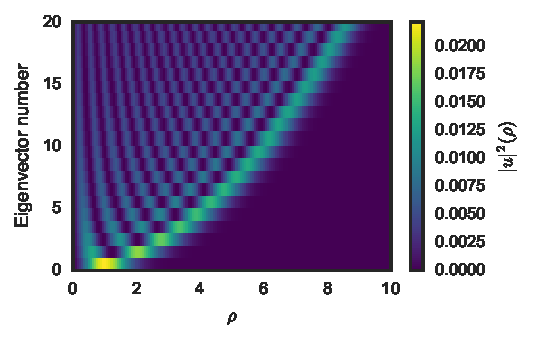
\includegraphics{eigenvecs.pdf}
            \caption{The probability distributions of the first 20 eigenfunctions of the one-electron system. The distributions are plotted as a function of $\rho$ from left to right, and distributions with increasing energy are plotted from bottom to top. The color corresponds to the magnitude of the probability distribution at each point.}
            \label{fig:eigvecs}
        \end{figure}

        To check whether the program is correct, the eigenvalues and eigenvectors were compared to those found by a divide-and-conquer eigenvalue algorithm provided by the function \texttt{eig\_sym} from the Armadillo C++ linear algebra library \cite{Sanderson2010}. The first 20 eigenvalues differ between the two codes by $10^{-7}$ at most, which is within the limits of floating-point precision. The probability distributions produced by the algorithm from Armadillo differ from those produced by the Jacobi algorithm by $10^{-10}$ at most, which implies a difference on the order of $10^{-5}$ in the magnitude of the eigenvectors. Assuming the results from the Armadillo library are correct, this confirms that the Jacobi algorithm is implemented correctly in this code.

    \subsection{Two-electron case}
    \label{sub:twoelecresults}
        The Jacobi algorithm code was run with the two-electron potential $\omega_r^2 \rho^2 + (1/\rho)$ for four values of $\omega_r$: 0.01, 0.5, 1.0, and 5.0. Once again, the maximum value of $\rho$ was set to 10, and the number of grid points was $375$. The probability distributions corresponding to the lowest three eigenvalues produced by the code are shown in Figure~\ref{fig:wavefunctions} with the corresponding one-electron distributions for comparison. The one- and two-electron distributions are very similar when $\omega_r = 1.0$ since the two potentials only differ by the addition of the $1/\rho$ term in that case. Otherwise, we can see that the electron distribution is pushed to higher values of $\rho$ as $\omega_r$ decreases. This is because a small value of $\omega_r$ allows the $1/\rho$ term to dominate the potential. On the other hand, a strong oscillator potential (large $\omega_r$) will dominate the Coulomb repulsion and drive the distribution toward smaller values of the separation $\rho$.

        The accuracy of the algorithm for the two-electron case can be compared to an exact analytic solution to the problem found by \textcite{Taut1993}. The code was run for three different values of $\omega_r$ which had analytic results listed in Taut. The results of this comparison are shown in Table~\ref{tab:exact}. The Jacobi code reproduced the analytic eigenvalues almost exactly.

        \begin{table}
            \begin{tabular}{S[table-format=1.5]
                            S[table-format=2]
                            S[table-format=1.4]
                            S[table-format=1.4]
                            S[table-format=1.4]}
                \hline\hline
                {$\omega_r$} & {$\rho_\text{max}$} & {Exact} & {Calculated} & {Difference} \\
                \hline
                0.25    & 10 & 1.250  & 1.250  & 0.000  \\
                0.05    & 15 & 0.3500 & 0.3510 & 0.0010 \\
                0.01827 & 30 & 0.1644 & 0.1644 & 0.0000 \\
                \hline\hline
            \end{tabular}
            \caption{Comparison of calculated eigenvalues of the two-electron system to an analytic solution for three values of the parameter $\omega_r$. The exact values are from \textcite{Taut1993}. (Note that the solutions printed in \cite{Taut1993} are a factor of 2 less than the ones shown here. This is due to a difference in how the expressions are derived in that paper, and it has been accounted for already in this table.)}
            \label{tab:exact}
        \end{table}

    \subsection{Performance}
    \label{sub:perf}
        The Jacobi code was run for increasing numbers of grid points to measure the code's performance. The number of similarity transformations required to diagonalize the matrix grew as $O(1.647 N^2)$ to leading order, where $N$ is the number of grid points (or the dimension of the matrix). A quadratic fit to this data is shown in Figure~\ref{fig:transformScaling}.

        \begin{figure}
            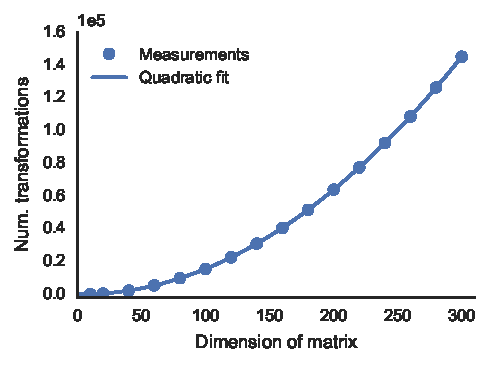
\includegraphics{transformScaling.pdf}
            \caption{Scaling of the number of similarity transformations required as a function of the dimension of the matrix. The fit shown is the quadratic function $N_\text{trans.} = \num{1.647}N^2 - \num{9.496} N + \num{7.899}.$}
            \label{fig:transformScaling}
        \end{figure}

        We also compared the time taken by the Jacobi code to that taken by the function from Armadillo. The time taken by each program was measured using the Unix \texttt{time} utility on a 2012 Mac Mini desktop computer with a \SI{2.3}{GHz} Intel Core i7 processor. The results are shown in Figure~\ref{fig:times} with power-law fits. The Jacobi algorithm was found to scale as $O(N^{3.814})$, while the algorithm from Armadillo scaled as $O(N^{1.817})$. The quality of this measurement is, however, limited by the fact that the \texttt{time} utility measures the execution time of the entire program, including the overhead for allocating and filling the matrices. The utility also only measures to a granularity of \SI{1}{ms}, so it cannot effectively measure the execution time of either algorithm for small $N$.

        \begin{figure}
            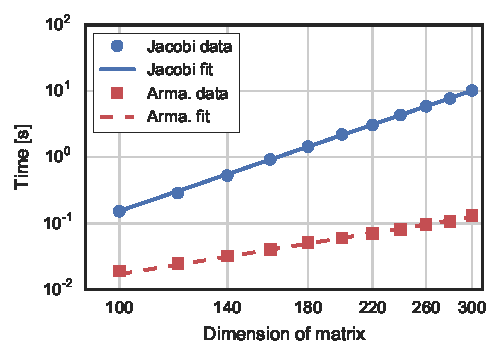
\includegraphics{timing.pdf}
            \caption{Time taken by each solver as a function of the dimension of the matrix, shown on a log-log scale. Each set of data was fit with a power law function $y=ax^b$. The fit shown for the Jacobi solver data is the function $t=(\num{3.60e-9}) N^{3.814}$, while the fit to the Armadillo data is $t=(\num{3.96e-6}) N^{1.817}$. Data for $N<100$ was not used since the times measured for these small values of $N$ were dominated by overhead and limited by the low precision of the Unix \texttt{time} utility.}
            \label{fig:times}
        \end{figure}

\section{Conclusion}
\label{sec:conclusion}
    While Jacobi's rotation algorithm is a straightforward and easily implemented method for finding the eigenvalues and eigenvectors of a matrix, it is also particularly slow and computationally inefficient. That was apparent in both the timing results, where this algorithm scaled as nearly a quartic function of the dimension of the matrix, and in the number of transformations performed, which scaled quadratically with the dimension of the matrix. Furthermore, the matrix being diagonalized here, which represented the Hamiltonian of one or two electrons confined to a harmonic potential well, was tridiagonal to begin with, which suggests that the algorithm could perform even worse for a general symmetric matrix.

    The performance of the algorithm could be improved by parallelizing parts of it. According to a time profile created by Apple's \emph{Instruments} program, the vast majority of the time spent in the algorithm is taken up by finding the largest off-diagonal element of the matrix. This would therefore be a good place to start with multithreading.

    That being said, the most obvious way to improve the performance of this process is to simply use a different, more efficient algorithm. The divide-and-conquer algorithm used by Armadillo's \texttt{eig\_sym} function would be a good candidate as its run time grew as $O(N^{1.817})$, which is significantly better than the Jacobi algorithm.

\bibliography{project2.bib}

\begin{figure*}
    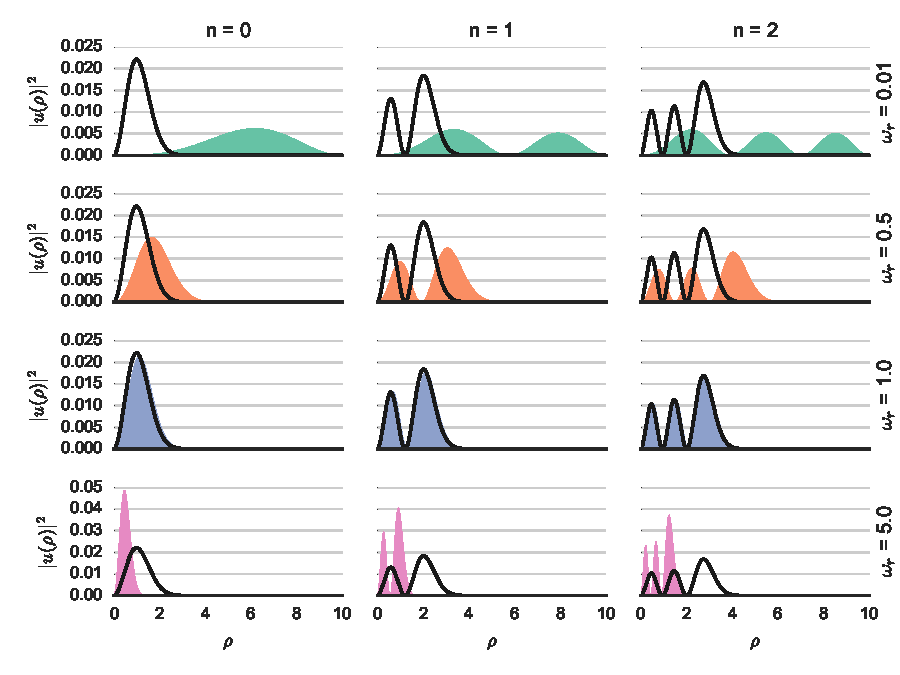
\includegraphics{wavefunctions.pdf}
    \caption{The three lowest-energy two-electron probability distributions for four values of $\omega_r$, plotted as the filled curves. The energy (or the magnitude of the eigenvalue) increases across columns from left to right, while the value of $\omega_r$ increases across rows from top to bottom. The solid black curve on each plot is the corresponding one-electron probability distribution. The one- and two-electron distributions are very similar for $\omega_r = 1.0$, but they diverge from each other as $\omega_r$ moves away from 1.0.}
    \label{fig:wavefunctions}
\end{figure*}

\end{document}
